\documentclass{beamer}

\usetheme{Frankfurt}

\usepackage[utf8x]{inputenc}
\usepackage[ngerman]{babel}
\usepackage{subfigure}
\usepackage{caption}
\usepackage{listings}
\usepackage{hyperref}

\lstdefinelanguage{diff}
{
    morekeywords={+, -},
    sensitive=false,
    morecomment=[l]{//},
    morecomment=[s]{/*}{*/},
    morecomment=[l][\color{darkgreen}]{+},
    morecomment=[l][\color{red}]{-},
    morestring=[b]",
}


% draw
%\usepackage[rgb]{xcolor}
\definecolor{hublue}{rgb}{  0, .21, .42}
\definecolor{darkred}{rgb}{.5, 0, 0}
\definecolor{darkgreen}{cmyk}{0.7, 0, 1, 0.5}
\definecolor{darkblue}{rgb}{0, 0, .5}

\usepackage[lflt]{floatflt}

\setbeamertemplate{footline}{%
  \usebeamerfont{date in head/foot}
%  \insertshortauthor - \inserttitle{}\hfill
%  \usebeamertemplate{navigation symbols}\hfill
  \insertframenumber{}/\inserttotalframenumber}
\setbeamertemplate{sidebar right}{}


\title{SAFERTOUCH}
\institute[{Humboldt-Universität zu Berlin}]{\inst{}Humboldt-Universität zu Berlin}
\author[Magnus Müller \and Kai Warncke \and Dominik Oepen]{Magnus Müller \and Kai Warncke \and Dominik Oepen}
\date[16.02.2011]{16. Februar 2011}

\begin{document}
%%%%%%%%%%%% Teil Dominik
	\begin{frame}
		\titlepage
	\end{frame}

	\begin{frame}
		\frametitle{Gliederung}
		\tableofcontents
	\end{frame}	

  \section{Motivation}
	\begin{frame}
		\frametitle{Motivation}
		\begin{block}{SOSEWIN-Vision}
		\begin{itemize}
			\item EFWS mit hunderten bis tausenden Knoten
			\item Idealfall: Nutzer installieren selbst Knoten bei sich zu Hause
			\item Knoten müssen dem Endnutzer Mehrwert bieten
		\end{itemize}
		\end{block}
		\pause
		\begin{block}{Mögliche Zusatzdienste}
			\begin{itemize}
				\item Heimautomatisierung
				\item Community-Dienste
				\item Location-based Services
			\end{itemize}
		\end{block}
		\pause
		Benötigt Ein-/Ausgabemöglichkeiten: Touchscreen
	\end{frame}

	\begin{frame}
		\frametitle{Mimo 720f}
		\begin{center}
			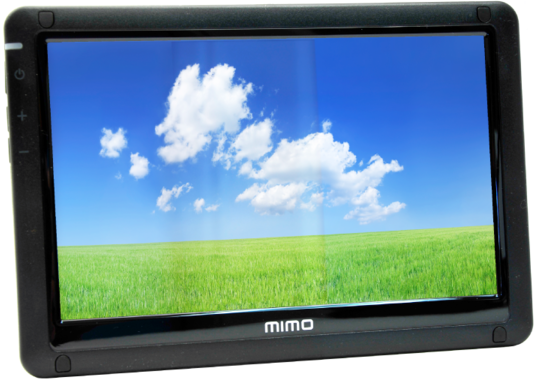
\includegraphics[scale=0.3]{img/mimo720f}
		\end{center}
		
		\begin{itemize}
			\item 7 Zoll Bildschirmdiagonale, Auflösung 800*480
			\item USB-Powered
			\item Displaylink-Chip (USB auf DVI)
			\item Touchscreen (e2i)
		\end{itemize}
	\end{frame}

	\section{Displaylink}
	
	\begin{frame}
		\frametitle{Displaylink}
		\begin{itemize}
			\item Chipsätze zur Konvertierung von USB nach DVI
			\item Serien DL-1x5 und DL-1x0
			\item Verwendet in Geräten unterschiedlicher Hersteller (u.a. Samsung, Nanovision)
        	\item Ansteuerung über Framebuffertreiber (udlfb) oder X-Server
		\end{itemize}	
	\end{frame}	

%  \subsection{Technische Details}
%	\begin{frame}
%		\frametitle{Displaylink}
%		\begin{itemize}
%			\item Stromchiffre zur Verschlüsselung der Daten (LFSR)
%			\item Sehr effiziente Huffman-Codierung zur Kompression
%			\item Reverse Enigeering durch Florian Echtler und Chris Hodges \footnote{Reverse-Engineering DisplayLink devices -- USB to DVI for hackers \url{http://events.ccc.de/congress/2009/Fahrplan/events/3353.en.html}}
%			\item (Eingeschränkte) freie Treiber von Displaylink
%			\item Offene Treiber aus der OSS Community
%		\end{itemize}
%	\end{frame}	
	
	\begin{frame}
		\frametitle{udlfb I}
		\begin{itemize}
			\item Kerneltreiber um Displaylink Geräte als Framebuffer zu verwenden
			\item Reverse-Engineering von Displaylink-Chips durch Florian Echtler und Chris Hodges
			\item Juni 2009 in Staging-Zweig des Kernel aufgenommen (2.6.31)
			\item November 2010 in Hauptzweig übernommen (2.6.37), erscheint ab 2.6.38 in mainline kernel
		\end{itemize}
	\end{frame}	

	\begin{frame}
		\frametitle{udlfb II}
		\begin{itemize}
			\item Kerneloption: \lstinline{CONFIG_UDLFB}
			\item Anschließend kann Display als \lstinline{/dev/fbX} angesprochen werden
			\item Benötigt angepasste Software
		\end{itemize}
		\pause
		\begin{center}
			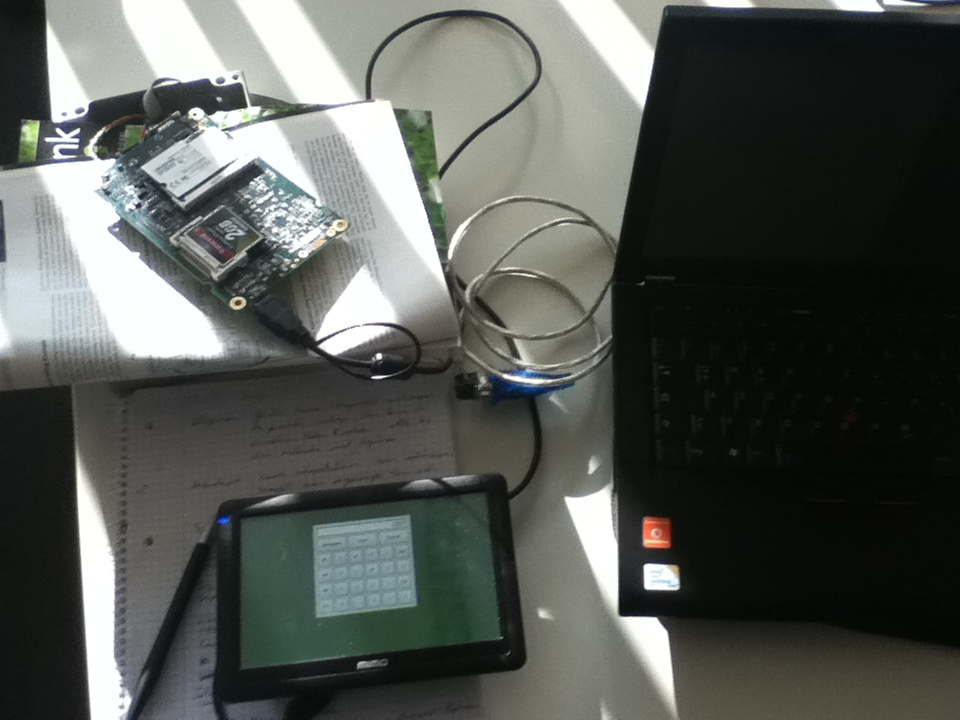
\includegraphics[scale=0.2]{img/mimo_hacking_1.jpg}
		\end{center}
	\end{frame}
			
	\begin{frame}
		\frametitle{Mimo 720f und OpenWRT}
    \begin{block}{Backfire}
    	\begin{itemize}
	    	\item Backfire-Kernel (2.6.32.27) enthält udlfb
    		\item Alte Version $\Rightarrow$ schlechte Performance
    		\item Keine Unterstützung für Touchscreen
    	\end{itemize}
    \end{block}
    \begin{block}{Zwei Lösungsansätze}
		\begin{enumerate}
			\item Neueren Kernel in Backfire einbinden
			\item OpenWRT Developer-Branch nutzen
		\end{enumerate}
    \end{block}
	\end{frame}
	
%%%%%%%%%%%% Teil Magnus
  \section{Touchscreen}
	
	\begin{frame}
		\frametitle{Touchscreen}
		%% Getrennt von Framebuffer
		%% evtouch (X.org)
		%% Kerneltreiber e2i
		%% tslib zur Kalibrierung
    \begin{block}{Anbindung des Touchscreen}
    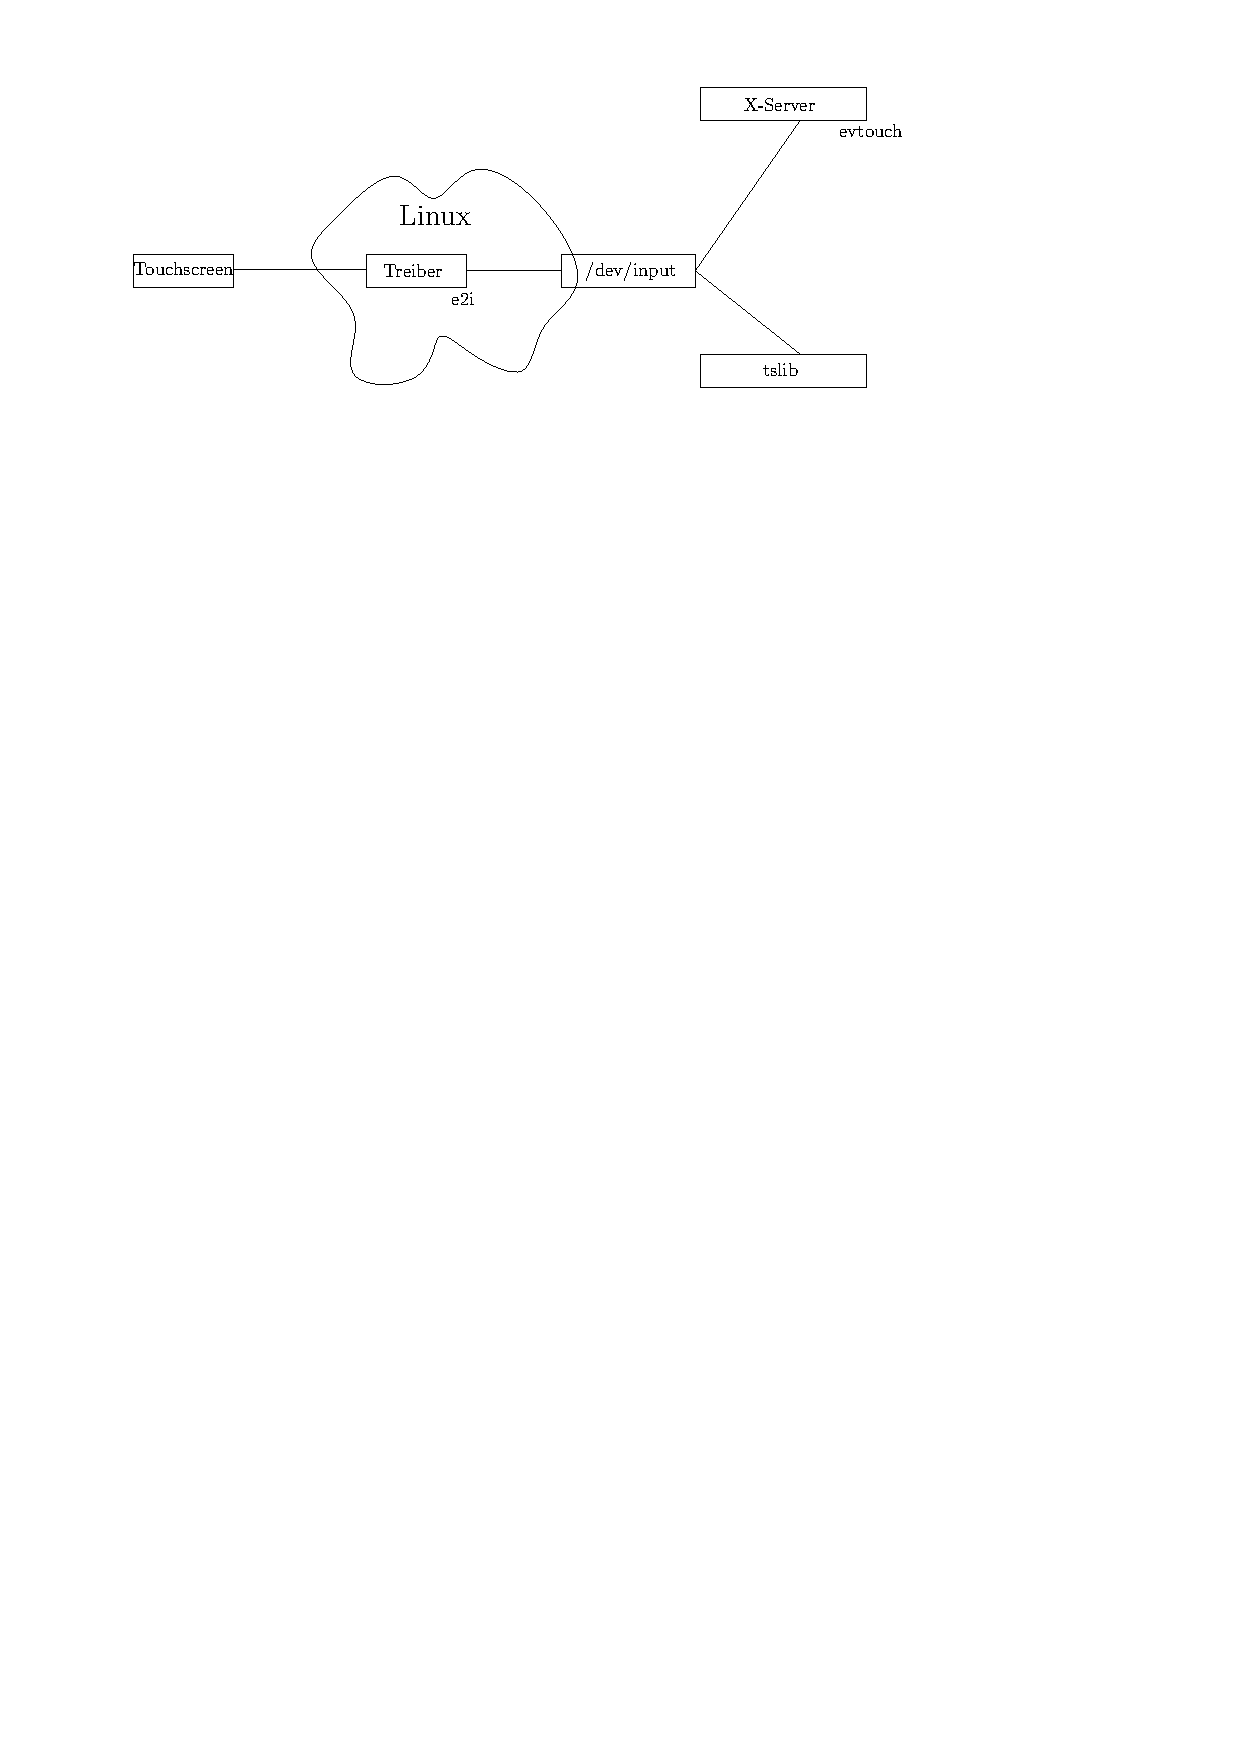
\includegraphics[width=\textwidth]{img/touchscreen/uebersicht.pdf}
    \end{block}
	\end{frame}	
	
	\section{Qt}
	
	\begin{frame}[containsverbatim, squeeze]
  \label{ioctl}
  %% Motivation fuer Verwendung von Qt
  %% Und: Kleine Demo dass das Teil auch funktioniert.
  \frametitle{Direkter Umgang mit Framebuffer ist mühsam}
		\begin{lstlisting}[language=C, basicstyle=\scriptsize]
/* fd wurde per open initialisiert */
struct fb_var_screeninfo screen;
ioctl(fd, FBIOGET_VSCREENINFO, &screeninfo);

int width = screeninfo.xres;
int height = screeninfo.yres;

__u16 *data = (__u16 *) mmap (0, width*height*2, 
                PROT_READ|PROT_WRITE, MAP_SHARED, fd, 0);

for (int row = 0; row < height; row++) {
    for (int column = 0; column< width; column++) {
        data[column+row*width] = 0xe111;
    }
}

int coords[4] = {0, 0, screen.xres_virtual, screen.yres_virtual};

if (ioctl (fd, DL_IOCTL_BLIT, &coords) == -21) 
    fprintf (stderr, "Error on ioctl call.\n");

munmap (data, width*height*2);
		\end{lstlisting}
    \hyperlink{backtoqt}{-}
	\end{frame}	
	
	\begin{frame}
		\frametitle{Qt}
		\begin{floatingfigure}[l]{1.75cm}
			
\includegraphics[scale=0.3]{img/qt-logo}
		\end{floatingfigure}
    \begin{itemize}
      \item Framework für Applikations- und Nutzerschnittstellen
      \item Freie Lizenz (LGPL)
      \item Weit verbreitet 
      \item Unterstützt eingebetteten Architekturen
      \item Integrierte Entwicklungstools
      \item Klein auf eingebetteten Architekturen (13 Mb gepackt inklusive
        Beispielsammlung)
    \end{itemize}
	\end{frame}	

  \begin{frame}
    \frametitle{QtCreator}
    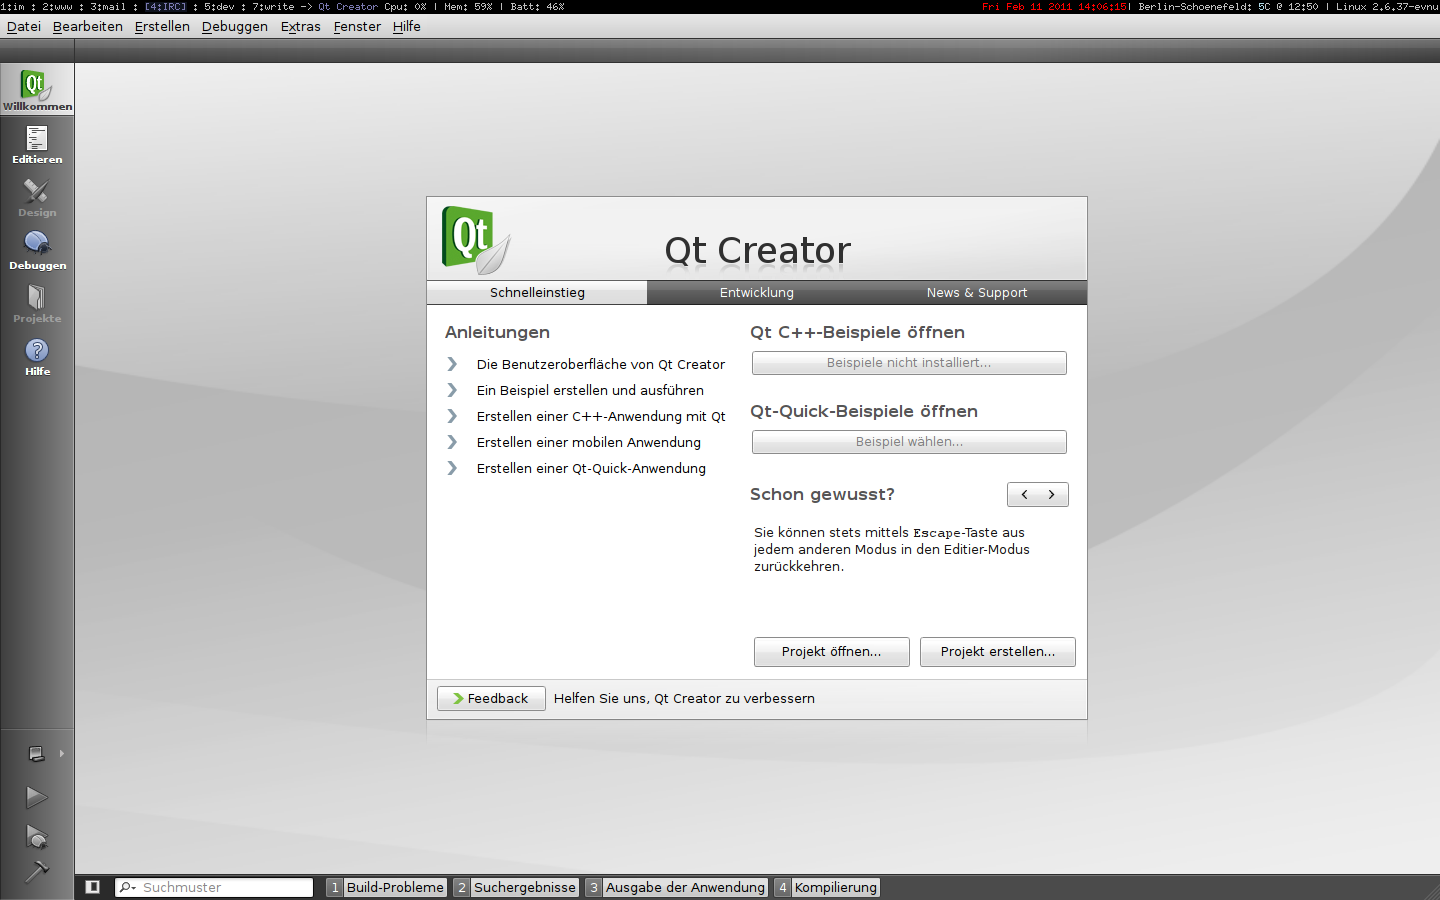
\includegraphics[scale=0.2]{img/qtcreator.png}
  \end{frame}
	
	\begin{frame}
		\frametitle{Qt und Mimo}
    \begin{block}{Framebuffer \& Qt}<1->
      \begin{itemize}
        \item<2-> Qt enthält Framebufferunterstützung (linuxfb und directfb)
        \item<4-> Funktioniert nicht mit udlfb
        \item<5-> Grund: Fehlender \hyperlink{ioctl}{\beamergotobutton{ioctl}}
          \hypertarget{backtoqt}{} zur Aktualisierung des Bildschirminhalts 
      \end{itemize}
    \end{block}
    \begin{block}{Touchscreen \& Qt}<1->
        \begin{itemize}
          \item<3-> Qt enthält Touchscreenunterstützung (LinuxInput, tslib, \ldots)
          \item<6-> Funktioniert nicht out-of-the-box mit e2i
          \item<7-> Grund: Kalibrierung von tslib ist nötig und Umgebungsvariablen müssen gesetzt
            werden.
        \end{itemize}
    \end{block}
	\end{frame}
	
  \subsection{Framebuffer}
  \begin{frame}
    \frametitle{Framebufferintegration in Qt}
    \begin{itemize}
      \item QWS (Q Windowing System)
      \item qscreenlinuxfb
    \end{itemize}
  \end{frame}
	\begin{frame}[containsverbatim, allowframebreaks, squeeze]
		\frametitle{Qt patch für udlfb}
		\begin{lstlisting}[language=diff, basicstyle=\tiny]
--- qscreenlinuxfb_qws.h.org	2011-02-04 16:12:27.000000000 +0100
+++ qscreenlinuxfb_qws.h	2011-02-04 16:23:11.241035001 +0100
@@ -88,7 +88,7 @@
 
     virtual bool useOffscreen();
 
-    enum DriverTypes { GenericDriver, EInk8Track };
+    enum DriverTypes { GenericDriver, EInk8Track,  UDLFB};
 
     virtual void disconnect();
     virtual void shutdownDevice();	
     
     
     
     
     
     
     
     
     
     
     
     
     
     
     
     
     

--- qscreenlinuxfb_qws.cpp.org	2011-02-04 16:11:34.000000000 +0100
+++ qscreenlinuxfb_qws.cpp2011-02-04 16:20:39.741035002 +0100
@@ -337,7 +337,12 @@
         return false;
     }
 
-    d_ptr->driverType = strcmp(finfo.id, "8TRACKFB") ? GenericDriver : EInk8Track;
+    if (!strcmp(finfo.id, "8TRACKFB"))
+        d_ptr->driverType = EInk8Track;
+    else if (!strcmp(finfo.id, "udlfb"))
+        d_ptr->driverType = UDLFB;
+    else
+        d_ptr->driverType = GenericDriver;
 
     if (finfo.type == FB_TYPE_VGA_PLANES) {
         qWarning("VGA16 video mode not supported");
@@ -1252,6 +1257,9 @@
             ioctl(d_ptr->fd, 0x46a2, 1);
         else
             ioctl(d_ptr->fd, 0x46a2, 0);
+    } else if (d_ptr->driverType == UDLFB) {
+        int coords[4] = {r.left(), r.top(), r.right(), r.bottom()};
+        ioctl(d_ptr->fd, 0xAA, &coords);
     }
 }
		\end{lstlisting}
	\end{frame}

  \subsection{Touchscreen}
  \begin{frame}
    \begin{center}
    Bleibt nur noch Touchscreen\ldots
    \end{center}
  \end{frame}
	\begin{frame}[containsverbatim, allowframebreaks]
    \frametitle{Umgang mit tslib}
    \begin{block}{Umgebungsvariablen}
      \begin{lstlisting}[language=Bash]
export TSLIB_CONSOLEDEVICE=none
export TSLIB_FBDEVICE=/dev/fb0
export TSLIB_TSDEVICE=/dev/input/event0
export TSLIB_CALIBFILE=/etc/pointercal
export TSLIB_CONFFILE=/etc/ts.conf
export TSLIB_PLUGINDIR=/usr/lib/ts
export QWS_MOUSE_PROTO=tslib:/dev/input/event0
      \end{lstlisting}
    \end{block}
    \begin{block}{Kalibrierung}
      \begin{lstlisting}[language=Bash]
        tests/ts_calibrate
      \end{lstlisting}
    \end{block}
    \begin{block}{Preload}
      \begin{lstlisting}[language=Bash]
LD_PRELOAD=/usr/lib/libts.so executable -qws
      \end{lstlisting}
    \end{block}
  \end{frame}

	\begin{frame}
		\frametitle{Ausgabe}
		\begin{center}
			\Huge{Fragen ?}
		\end{center}
		\begin{center}
			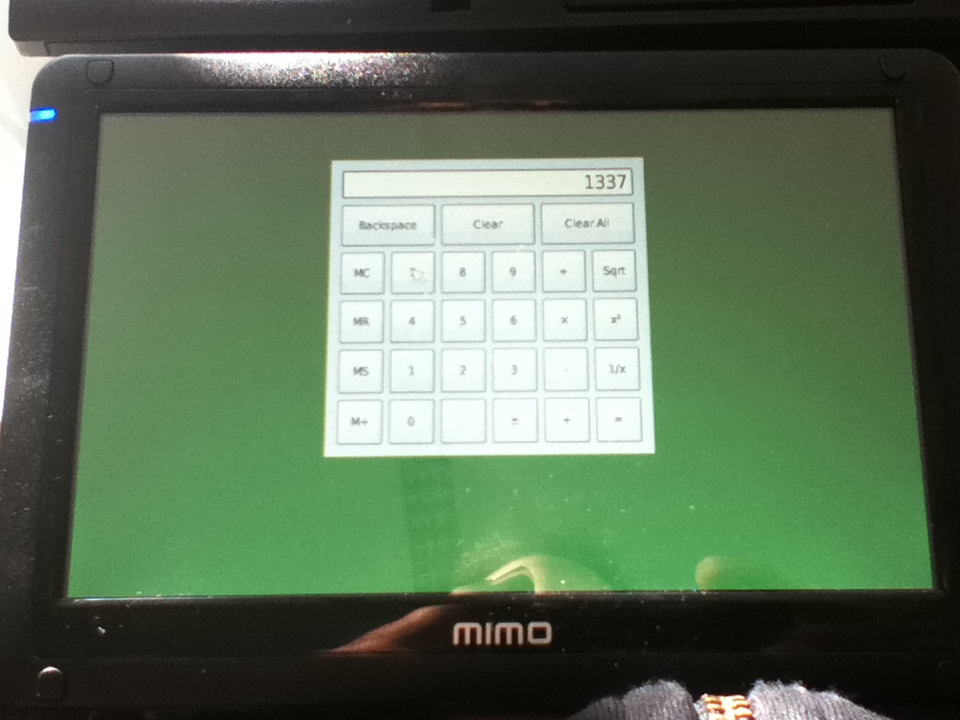
\includegraphics[scale=0.2]{img/mimo_calc.jpg}
		\end{center}
	\end{frame}

\end{document}
